\section{FPCCD}
\subsection{Collaborating Institutions}
\subsection{Introduction}
    Fine pixel CCD (FPCCD) is one of the candidate sensor options for the vertex detector of the ILD detector at the ILC~\cite{Sugimoto:2005ru,2009arXiv0902.2067S,2012arXiv1202.5832S}. In the present design, FPCCD sensors for the innermost layer of the vertex detector have a pixel size of \unit[5]{\micron} and a fully depleted epitaxial layer with a thickness of \unit[15]{\micron}. Because of the small size of the pixels, the occupancy is acceptably low even if the hits are accumulated for one nominal ILC bunch train (\unit[~1]{ms}).
    The efforts of the FPCCD collaboration are currently focused on pixel characterization and development, while we also pursue developments to the cooling system, electronics downstream of ASICs and the reconstruction software~\cite{Mori:2014xta}.
\subsection{Recent Milestones}
R\&D activity for the FPCCD vertex detector at present is mainly focused on FPCCD sensors and a detector cooling system using 2-phase \ce{CO2}.  
One of the achievements of FPCCD sensors after DBD is the fabrication of real size ($12.3 \times \unit[62.4]{\mathrm{mm}^2}$) sensors with \unit[50]{\micron} total thickness. Figure~\ref{fig:FPCCD:realSizeSensor} shows the real size prototype sensor. It has 8 readout nodes, and each channel has different pixel sizes of \unit[12]{\micron}, \unit[8]{\micron}, and \unit[6]{\micron}.
\begin{figure}
    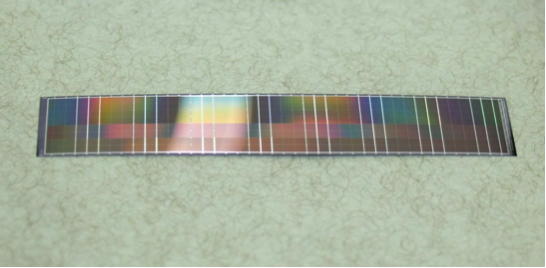
\includegraphics[width=\textwidth]{VertexDetector/FPCCD/realSizeFPCCDSensor.png}
    \caption{Real size FPCCD sensor thinned down to \unit[50]{\micron}}
    \label{fig:FPCCD:realSizeSensor}
\end{figure}
We have started a neutron damage test using small ($\unit[6]{mm}\times\unit[6]{mm}$) FPCCD prototypes~\cite{lcws:fpccd:ito:2013}. A prototype sensor was irradiated by a neutron beam of few tens of MeV at the CYRIC facility of Tohoku University. The detailed analysis on the irradiated sensor is still on-going.
In order to increase the radiation immunity of FPCCD sensors, particularly to reduce the transfer inefficiency due to radiation damage, the sensors should be cooled down to \unit[-40]{\degree C}. We have started R\&D on a two-phase \ce{CO2} cooling system for this purpose. There are several examples of utilizing two-phase \ce{CO2} cooling systems for high energy physics experiments. For these cases, the \ce{CO2} coolant is circulated using liquid pumps. This method is, however, not so efficient for very low temperature cooling of \unit[-40]{\degree C}. Therefore, we adopted a \ce{CO2} gas compressor for the circulation of \ce{CO2} coolant. Figure~\ref{fig:FPCCD:coolingSystemSchematic} shows a simplified schematic diagram of the system. A prototype system has been constructed, and cooling between \unit[-40]{\degree C} and \unit[+15]{\degree C} has been successfully demonstrated using this system.
\begin{figure}
    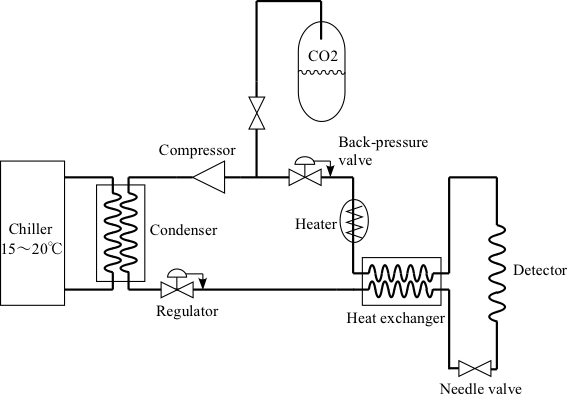
\includegraphics[width=\textwidth]{VertexDetector/FPCCD/coolingSystemSchematic.png}
    \caption{A simplified schematic diagram of the two-phase $\text{CO}_2$ cooling system}
    \label{fig:FPCCD:coolingSystemSchematic}
\end{figure}

\subsection{Engineering Challenges}
    In the present design of the ILD vertex detector, two sensor layers are mounted on both sides of a light-weight ladder of ~\unit[2]{mm} thickness. Our goal of the material budget of this ladder is 0.3\% X0/ladder = 0.15\% X0/layer. This goal would not be so easy to accomplish, and we need a lot of R\&D effort.
    The ladders have to be cooled down to \unit[-40]{\degree C}. We plan to achieve this cooling by heat conduction to the end-plate on which thin cooling tubes for 2-phase \ce{CO2} are attached. The design of this structure is not trivial, and we need R\&D including thermal simulation.
    There are challenges both with the mechanical structure and the electronics circuit for the ladder R\&D. We have not started this effort yet.
\subsection{Future Plans}
    We have been doing our R\&D on the FPCCD vertex detector based on a Grant-in-aid for science research which expires at the end of FY2015. By that time, we plan to carry out the following R\&D items:
\begin{itemize}
    \item Characterization of FPCCD sensors including beam tests and radiation damage tests
    \item Development of FPCCD sensors with the pixel size of \unit[5]{\micron}, which is our ultimate goal
    \item Construction of prototype ladders for inner layers
    \item Development of readout electronics downstream of ASICs
\end{itemize}
If new funding is secured in future, the following R\&D items have to be done:
\begin{itemize}
    \item Development of larger FPCCD sensors and prototype ladders for outer layers
    \item Development of readout electronics which can fit in the small space of real experiment
    \item Construction of a real size engineering prototype and its cooling test
\end{itemize}

\subsection{Applications Outside of Linear Colliders}
    Because of the relatively slow readout speed, the application of FPCCD sensors to other high energy physics experiments would be limited. However, high spatial resolution of small pixel size must be applicable to measurements of X-ray imaging.
    Two-phase \ce{CO2} cooling system can be applied to any other detectors which require efficient cooling between \unit[-40]{\degree C} and near room temperature. Our system, which uses a \ce{CO2} gas compressor, has a great advantage for low temperature operation near \unit[-40]{\degree C} compared with systems using liquid pumps for circulation.

